\section{Proposal}

In this section, we propose {\model}, a novel automated metric to
evaluate SMT-based code migration tools. It is aimed to support source
code, and language-independent
%, and can reflect well the semantic
%accuracy of translated results, and inexpensive to compute. 
{\model} is then empirically validated on SMT-based code migration
models to show its effectiveness. 


\subsection{Design}

%\emph{Insight 1 :} 
According to Table~\ref{table:correlation} in Section 6, we can
observe a trend of increasing correlation coefficients with Semantic
scores when higher levels of representations are used for source code
from lexical tokens to AST, and to PDGs.
%
%there is a trend of increasing correlation coefficient with
%Semantic score when more complex level of source code's
%representations are used. 
Specifically, GVED has the highest correlation, and it is followed by
TREED and SED, respectively. 
% Tien
However, as explained earlier, we cannot use GVED as a sole metric to
evaluate the migrated code because {\em not all resulting migrated
  code is sufficiently correct to build the PDGs} and to compute
the feature vectors. 

To address this problem, we adapt an idea from machine learning,
called {\em ensemble methods}~\cite{ensemble}. In machine learning,
ensemble methods use multiple learning algorithms to obtain better
predictive performance than could be obtained from any of the
constituent learning algorithms alone~\cite{ensemble}.
% Tien
To apply to our problem, we would use the decision made by the most
reliable metric, which is GVED metric. In the case that the most
reliable metric is not available (due to the fact that an PDG cannot
be built from incorrectly migrated code), we would use the next
reliable one, which is TREED. TREED in turn would face the same issue
if the migrated code is not syntactically correct. In this case, we
would resolve to use SED as it is always computable for any given
piece of code with regard to the reference code. This design strategy
is reasonable because the probability of a translated method can be
built into PDG is lower than the probability that it is syntactically
correct because a segment of code needs to be compiled first before we
can build an PDG. On the other hand, SED can always be computed
regardless of the quality of migrated code and types of code migration
systems.

%Therefore, those metrics should have priority order when are used in
%evaluating translation results. The Expert System tries to address
%similar problem by inferring through a knowledge base of \lq if-then
%\rq rules, and using the best expert aarilable for the
%problem. Applying the Expert System's idea onto our problem, the best
%metric available should be used when evaluating translation result.


%\emph{Insight 2 :}
%For SMT-based Code Migration systems, a translated method cannot be guaranteed to be compilable or be built into PDG. It leads to the problems that GVED and TREED are not always applicable even though GVED is better than TREED, and TREED is better than SED. The probability of a translated method can be built into PDG is also lower than  the probability it can be compiled because a segment of code needs to be compiled first before building into PDG.  On the other hand, SED can always be computed regardless of translation result or types of Code Migration systems. To sum up, the 3 metrics have different advantages and disadvantages. Therefore, it is natural to combine the 3 metrics to overcome the disadvantages and boost the advantages. Indeed, there is a theory to backup that combination. In machine learning domain, Ensemble theory is to combine multiple classifiers to form a hopefully better one when each different classifier is more suited for a practical problem. 

From the above insight, we design {\model} as an ensemble expert-based
metric. {\model} is a combined metric that takes into consideration
metrics at the lexical, syntactical, and semantic levels of source
code while aiming to measure the semantic accuracy of translated code
in a reliable manner. {\model} utilizes the best metric available and
guarantees to give a reliable semantic accuracy regardless of
translation results. If the translated code can be built into PDG, we
calculate {\model} in term of graph vector edit distance (GVED). If
the translated code cannot be built into PDG, however it is
syntactically correct, {\model} is calculated as syntax tree edit
distance (TREED). Finally, if the translated code is not syntactically
correct, we take string edit distance (SED).

The formula to compute {\model} is presented in Algorithm~\ref{ruby}. GVED,
TREED, and SED were defined in Section~\ref{sec:alternatives}. $r$ is
the reference code, $t$ is the translated code; $r$ and $t$ are tokenized
into sequences to use in SED, are parsed into ASTs to use in TREED,
and are built into PDGs to use in GVED.  \makeatletter
\def\BState{\State\hskip-\ALG@thistlm} \makeatother
\begin{algorithm}
\caption{Calculate {\model}}\label{ruby}
\begin{algorithmic}[1]
\If { $\mbox{GVED}\left(r,t\right) $ is applicable }
\State $\mbox{RUBY}\left(r,t\right) = \mbox{GVED}\left(r,t\right) $
\ElsIf { $\mbox{TREED}\left(r,t\right) $ is applicable }
\State $\mbox{RUBY}\left(r,t\right) = \mbox{TREED}\left(r,t\right) $
\Else 
\State $\mbox{RUBY}\left(r,t\right) = \mbox{SED}\left(r,t\right) $
\EndIf
\end{algorithmic}
\end{algorithm}

\subsection{Proposal result}

To evaluate RUBY, we conducted the same experiment with other four
metrics to show the correlation of RUBY with semantic scores on two
model mppSMT and lpSMT. RUBY's efficiency was tested on a large number
of methods translated by those models.

\begin{figure}[t]
\caption{RUBY vs Semantic (lpSMT)}
\centering
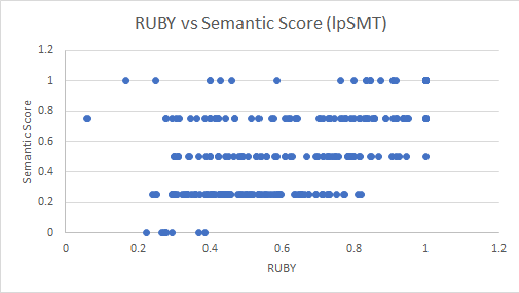
\includegraphics{img/rubyvssem_lpSMT.png}
\label{fig:RubySemlpSMT}
\end{figure}

\begin{figure}[t]
\caption{RUBY vs Semantic (mppSMT)}
\centering
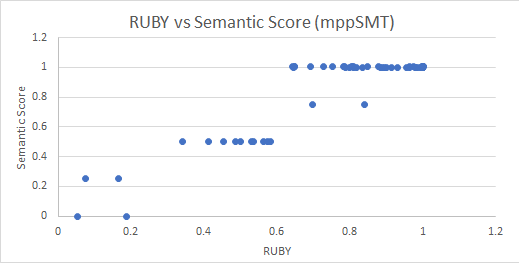
\includegraphics{img/rubyvssem_mppSMT.png}
\label{fig:RubySemMppSMT}
\end{figure}

Figures~\ref{fig:RubySemlpSMT} and~\ref{fig:RubySemMppSMT} show the
scatter plots between RUBY and Semantic scores on two models mppSMT
and lpSMT, respectively. As can be seen from the scatter plot for
lpSMT (Figure~\ref{fig:RubySemlpSMT}), there is a moderately strong,
positive, linear association between the two variables with a few
outliers.  Beside, the scatter plot for mppSMT
(Figure~\ref{fig:RubySemMppSMT}) shows a strong, positive, linear
association between RUBY and Semantic score. There are no outliers in
the data. This is the indication that the result is consistent.

In general, RUBY has high correlation with Semantic scores. As our
experiment result, the correlation coefficient between RUBY and
semantic score for model mppSMT is \textbf{0.862} and for the model
lpMSMP is \textbf{0.836}. In statistics, these values indicate a
strong uphill linear relationship between two quantitative
metrics. That means one metric could be predicted by the other with
high confidence. For example, an increase of 0.5, {\model} score can
be interpreted as an increase of 0.4 in term of Semantic score. Based
on that information, developers can tune the system in an incremental
manner.


%Specifically, a correlation of +0.8 implies that when 	

Although RUBY has a strong correlation coefficient, it is still lower
than GVED scores shown in Section~\ref{sec:alternatives} due to the
fact that only a subset of the dataset is applicable. While GVED is
only computed with the migrated code with sufficient semantic
information, RUBY does not depend on the code, even we can not parse
PDGs and ASTs. This implies that there exist a RUBY score for any
given code. On the other hand, in comparison with TREED, SED
and BLEU, RUBY always outperforms the other three metrics.
	    
  			




%BLEU has always been doing this and that....

%Researchers usually claim that an improvement in BLEU also meant an
%improvement in translation quality. So 

%BLEU has been used for not only evaluating the result but also tuning
%and developing SMT-based migration system.
%%From the results in section 5, BLEU did not reflect the semantic accuracy of source code. --> We need a better metrics to replace BLEU
%However, from the results in section 5, it can be concluded that BLEU
%did not reflect well the semantic accuracy of migrated source code
%since it has weak relation with human judgments. Therefore, we need a
%better metric in order to fit better with programming languages and
%code migration systems.
%%
%%Needed metric should be 
%%Reflect semantical meaning of sources code.
%%Automated
%%Low computation's cost
%%Independent of programming language
%%Independent of MT model's type
%Such a metric should have the following requirements:
%
%
%\emph{1}. The metric is more suitable for source code than BLEU. It
%can reflect the semantics of source code and the semantic accuracy of
%translation result. To fulfill that, the metric must have high
%correlation with human evaluation for the translation result.
%
%
%\emph{2}. The metric can be computed automatically and inexpensively in
%order to support the evaluation of migration results in the
%incremental development of SMT-based code migration systems. For
%example, the metric can be calculated quickly after each iteration of
%development so a system can be evaluated and tuned in a timely~manner.
%
%\emph{3}. The metric is independent of the programming languages and
%of the SMT models. A good and reliable metric must have consistent
%results for any languages and models so it can be applied universally
%to any SMT-based code migration systems.
%
%%What is Ruby and why Ruby is good.
%Considering all above requirements, we introduce {\model}, a novel automated metric that can reflect semantic accuracy of translated code. {\model} is also independent of programming languages and machine translation models used in migration system. {\model} measures the semantic accuracy of the resulting code with respect to reference code by comparing their Program Dependence Graph (PDG). PDG captures both the data and control dependencies among program entities. Because those dependencies play an important role in a program, we expect PDG can represent well the semantics of source code. Usually, comparing graph is expensive, but our approach makes it affordable. We estimate the graph edit distance by vectorizing the graph and calculating the vectors edit distance. Because of that, we can save the computational cost and make our approach scalable. Basically, every programming language code can be built into PDG. Hence, our metric can be used for Code Migration systems that migrate different programming languages. Lastly, the way {\model} is measured makes it independent of machine translation models. That means Code Migration systems that deployed different SMT models can still use our metric. Next, we go into details how to formalize the calculation of {\model}
%
%%To reduce the high computational cost, we vectorize the PDGs and calculate the vector difference to estimate the graph difference. This way, we would make sure that our model is practical and applicable in large scaled systems. 
%
%When applying MT on source code, there always exists the problem that the translated code is broken in term of syntax. Thus, it is impossible to build PDG or even compile those code. To cope with the problem, our model is designed as best-effort, layered metric  : If the translated code can be built into PDG, we calculate {\model} in term of graph edit distance. If the translated code cannot be built into PDG but is compilable, we calculate {\model} in term of syntax tree edit distance. If the translated code is not compilable, we calculate {\model} in term of string edit distance. We then represent about the 3 metrics graph/tree/string edit distances as follows:



